\subsection{Datenbank}

Als Datenbank wurde Firestore verwendet, ein Untermodul von Firebase, welches nutzern bis zu einem gewissen Umfang kostenlos zur Verfügung steht. Firestore ist eine NoSQL-Datenbank, welche auf Dokumenten basiert. Ähnlich wie bei MongoDB werden Daten als kleine Dokumente gespeichert, welche wiederum in Kollektionen gespeichert werden. Firestore erlaubt nesting, damit komplexere Datenstrukturen abgebildet werden können ohne, dass einzelnen Dokumente zu groß werden.


\subsubsection{Serialisierung / Deserialisierung}

Um die Daten der Datenbank auf der Seite des Tower Controllers zu verarbeiten, müssen diese zunächst in ein strukturiertes Format umgewandelt werden. Dies geschieht durch die Verwendung von \texttt{serde} und \texttt{serde\_json}. \texttt{serde} ist eine Bibliothek, welche es ermöglicht, beliebige Datenstrukturen zu serialisieren und deserialisieren. Es ist sehr einfach Datenstrukturen mittels \texttt{serde} serialiserbar zu machen.


\subsubsection{Datenbankschema}
Das Datenbankschema ist trotz der Verwendung einer Dokumenten-Datenbank änhlich zu relationalen Datenbanken. Aus diesem Grund kann das Schema der Datenbank auch als ER-Diagramm dargestellt werden.

\begin{figure}[H]
    \centering
    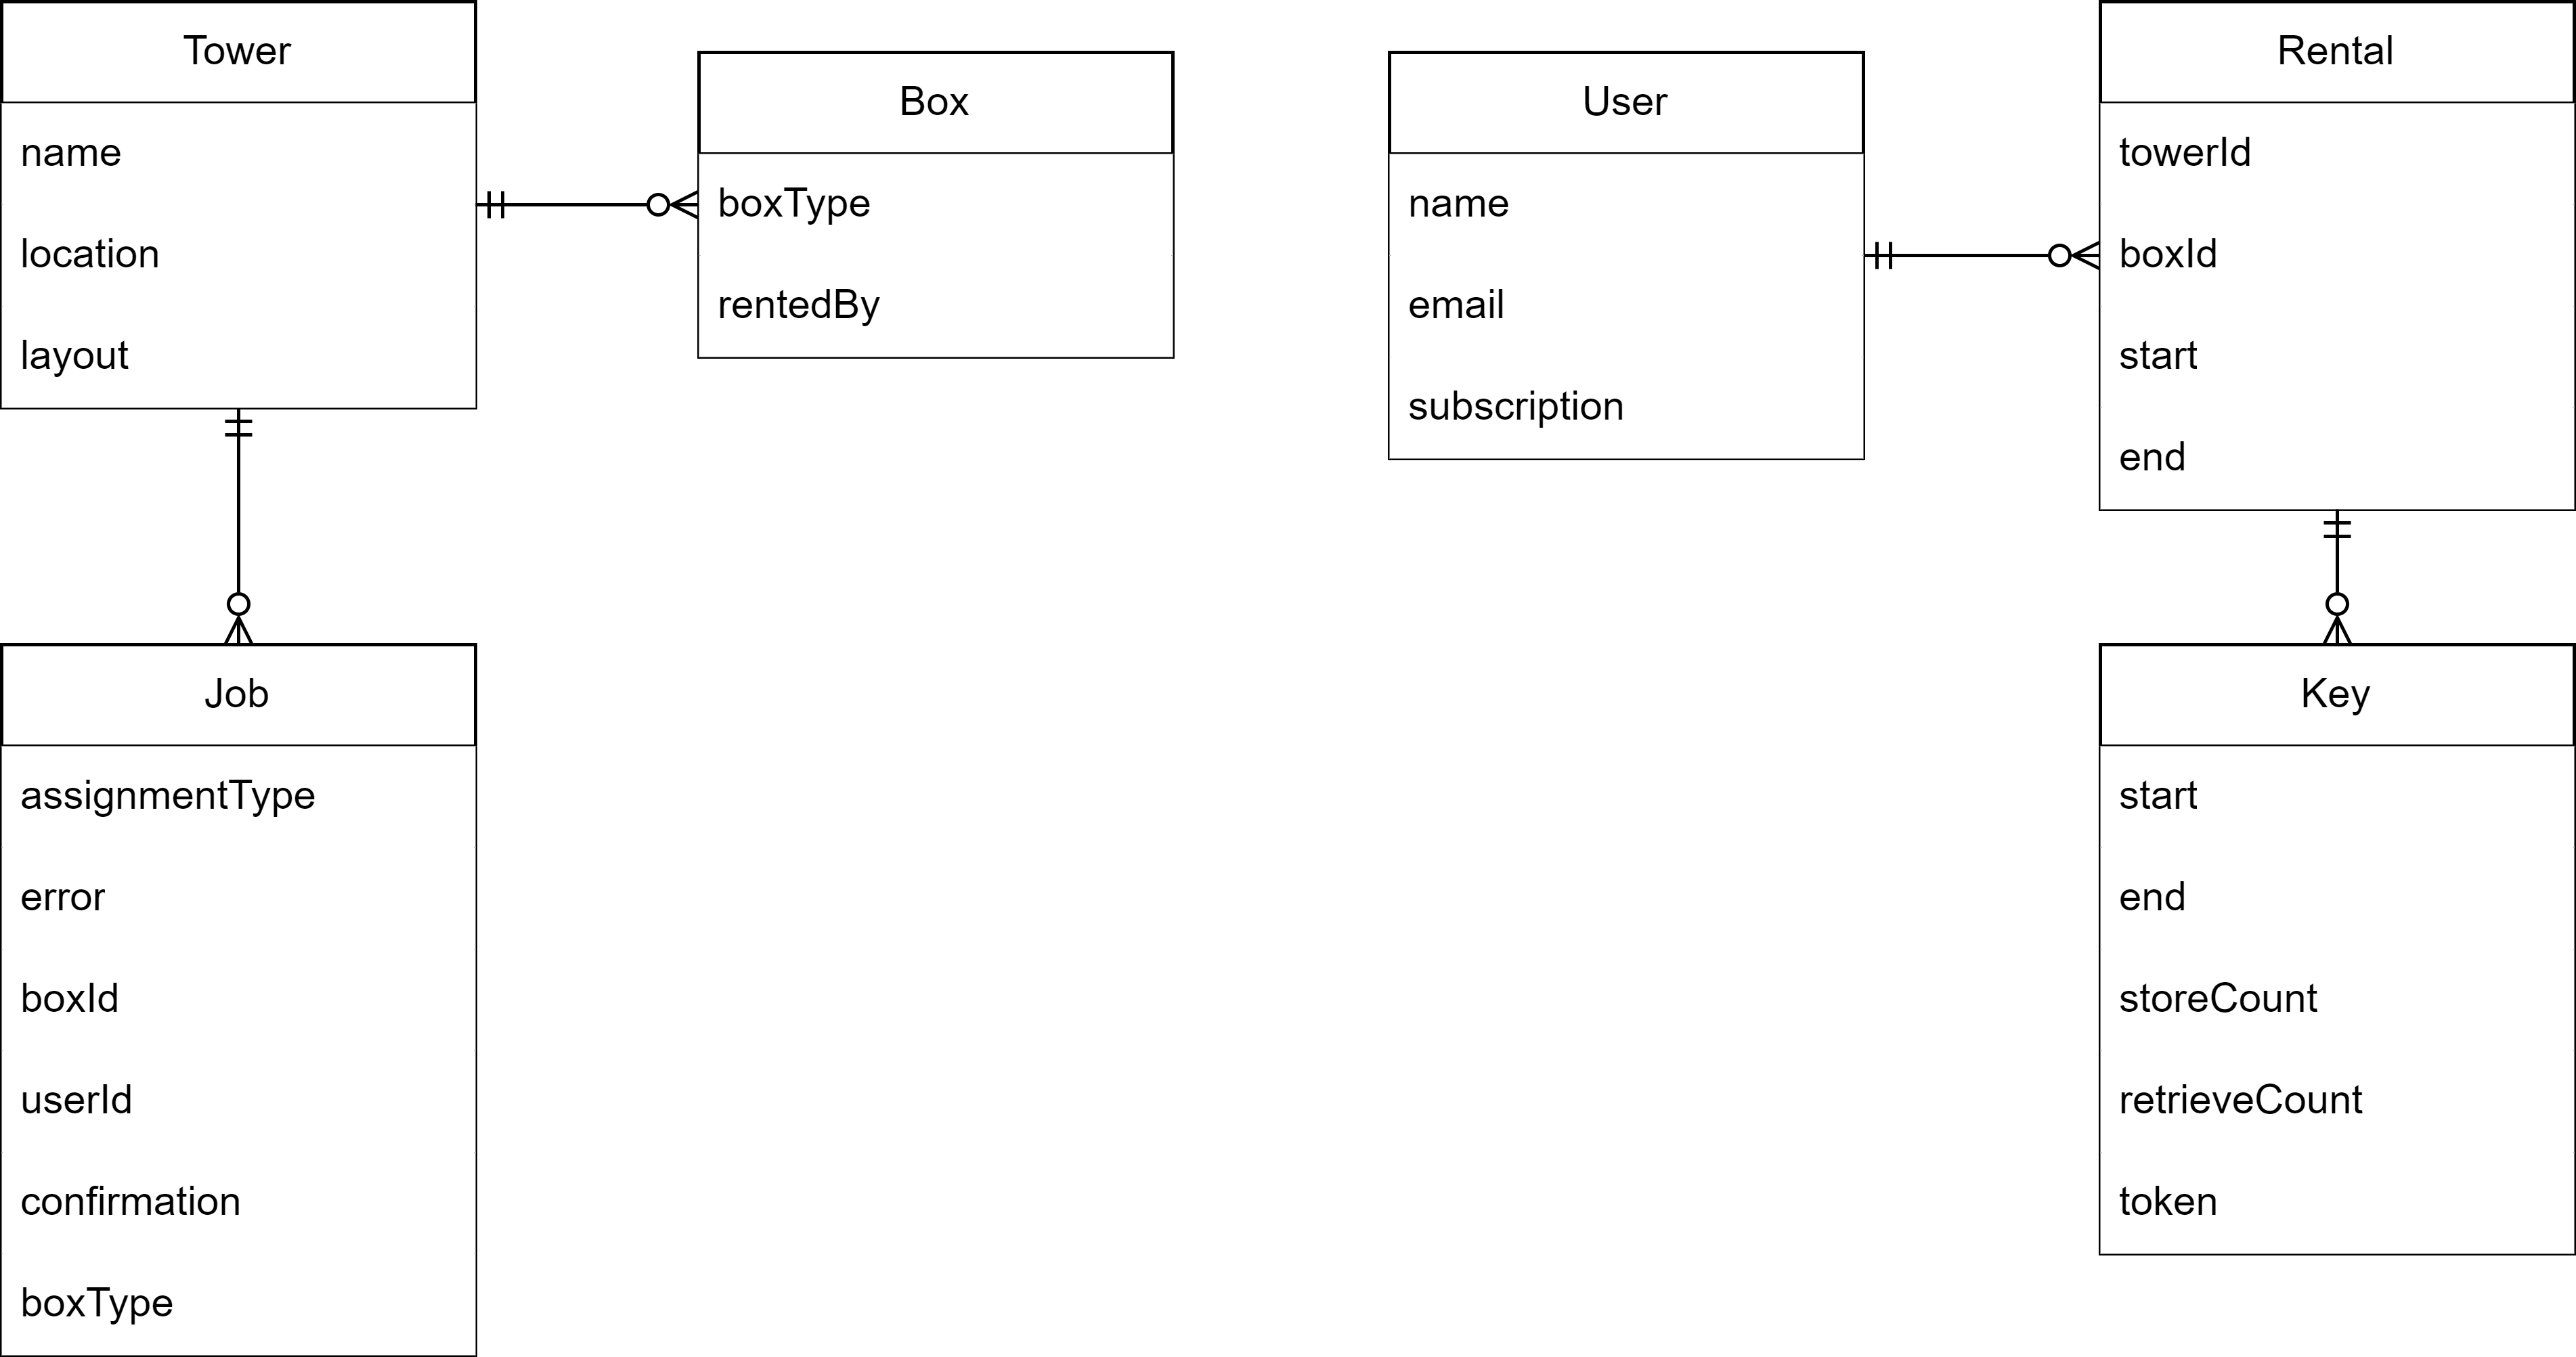
\includegraphics[width=0.9\textwidth]{images/datenbankstruktur.png}
    \caption{ER-Diagramm der Datenbank}
    \label{fig:er_diagramm}
\end{figure}

\paragraph{Tower}
Tower repräsentieren die einzelnen Standorte der Fahrradtürme. Sie enthalten die Koordinaten des Standortes, den namen des Standortes und die Kapazität des Standortes.

\begin{minted}{typescript}
Tower {
    layout: [number],
    location: LatLng,
    name: String,
}
\end{minted}

\paragraph{Box}
Eine Box repräsentiert einen einzelnen Lagerplatz bzw. Stellplatz im Fahrradturm. Sie enthalten die Art des Lagerplatzes und die ID des Nutzers, der den Platz aktuell nutzt (sofern der Stellplatz belegt ist).

\begin{minted}{typescript}
Box {
    boxType: "bike" | "item",
    rentedBy?: String,
}
\end{minted}


\paragraph{Job}
Jobs sind für die Kommunikation zwischen Turm und App verantwortlich. Sie enthalten Informationen über den Typ des Jobs, den Nutzer, der den Job anfrägt, die Box, die betroffen ist und den Status des Jobs. Je nach Typ des Jobs und Job-Fortschritt sind manche Felder nötigt oder leer.

\begin{minted}{typescript}
Job {
    assignmentType: "store" | "retrieve",
    error?: "noFreeSlots" | "invalidMessage" | "invalidPermissions" | ...,
    boxId?: String,
    userId: String,
    confirmation?: "jobRecieved" | "jobCompleted",
    boxType?: "bike" | "item",
}
\end{minted}


\paragraph{User}
User enthalten die Informationen über einen einzelnen Nutzer. Sie enthalten den Namen, die E-Mail-Adresse und den Status des Nutzers (ob er ein kostenpflichtiges Abo hat oder nicht).

\begin{minted}{typescript}
User {
    name: String,
    email: String,
    subscription: "free" | "premium"
}
\end{minted}


\paragraph{Rental}
Ein Rental repräsentiert einen einzelnen Verleihvorgang. Sie enthalten die ID des Turms, bei dem die Box gemietet wurde, die ID der Box, den Startzeitpunkt der Miete und den Endzeitpunkt der Miete (sofern die Miete bereits beendet ist).

\begin{minted}{typescript}
Rental {
    towerId: String,
    boxId: String,
    start: Timestamp,
    end?: Timestamp,
}
\end{minted}


\paragraph{Key}
Keys sind dafür da um Dritten Zugriff auf vermietete Boxen eines Nutzers zu gewähren. Je nach verwendungszweck kann ein ablaufdatum für den Key gesetzt werden. Zudem kann auch ein Limit für die Anzahl der Verwendungen gesetzt werden (separat für ein- und auslagerung). Keys werden zum Beispiel dazu verwendet um Paketlieferanten Zugriff auf die Boxen zu gewähren, damit diese ein Paket abliefern können.

\begin{minted}{typescript}
Key {
    start: Timestamp,
    end?: Timestamp,
    retrieveCount?: number,
    storeCount?: number,
    token: String,
}
\end{minted}